\chapter{Implementation}
\label{chapter:methods}

\section{Overview}
In this chapter, we start off by discussing the dataset used and what makes the dataset unique in Section \ref{section:bizspeech}. Then, we look at how to make the data usable for an \acrshort{asr} application with steps like forced alignment and audio normalization in Section \ref{section:dataprep}. Next, we go over the details for training the acoustic encoder decoder model used in Section \ref{section:attention_train}. Lastly, we explore the distributed methodologies used and discuss the practical choices taken when using those methods in Section \ref{section:di}



\section{Business Speech (BizSpeech) Dataset}
\label{section:bizspeech}
As mentioned in the Section \ref{section:largescale_related}, there are not many datasets which are available publicly for training speech recognition systems at a scale of around tens of thousands of hours. This section introduces Business Speech dataset, which has been used for all the experiments in this thesis. 

Business speech dataset consists of conference calls, which are corporate disclosure and brokerage event information. It can be accessed through a paid licence here\footnote{Company Events Coverage, StreetEvents, Refinitiv. \href{https://www.refinitiv.com/en/financial-data/company-data/company-events-coverage}{https://www.refinitiv.com/en/ financial-data/company-data/company-events-coverage}}. Refinitiv also provides transcriptions, call summaries and other metadata like date and PermID, which is the ID number for the firm. This ID can further be used to link to many more metadata information from other datasets like the officers and directors dataset\footnote{Officers and Directors data, Refinitiv \href{https://www.refinitiv.com/en/financial-data/company-data/officers-and-director-search}{https://www.refinitiv.com/en/financial-data/ company-data/officers-and-director-search}} which provides information about the firm's financials, personnel involved etc. The audio and transcripts can be accessed via APIs and also via the Eikon software\footnote{Eikon Financial Analysis \& Trading Software, Refinitiv \href{https://www.refinitiv.com/en/products/eikon-trading-software}{https://www.refinitiv.com/ en/products/eikon-trading-software}} \cite{August2011ThomsonEikon}. Figure \ref{fig:eikon} shows a snapshot of the software in use.

\begin{figure}[ht]
  \begin{center}
    % below the size of the figure has been reduced for example
    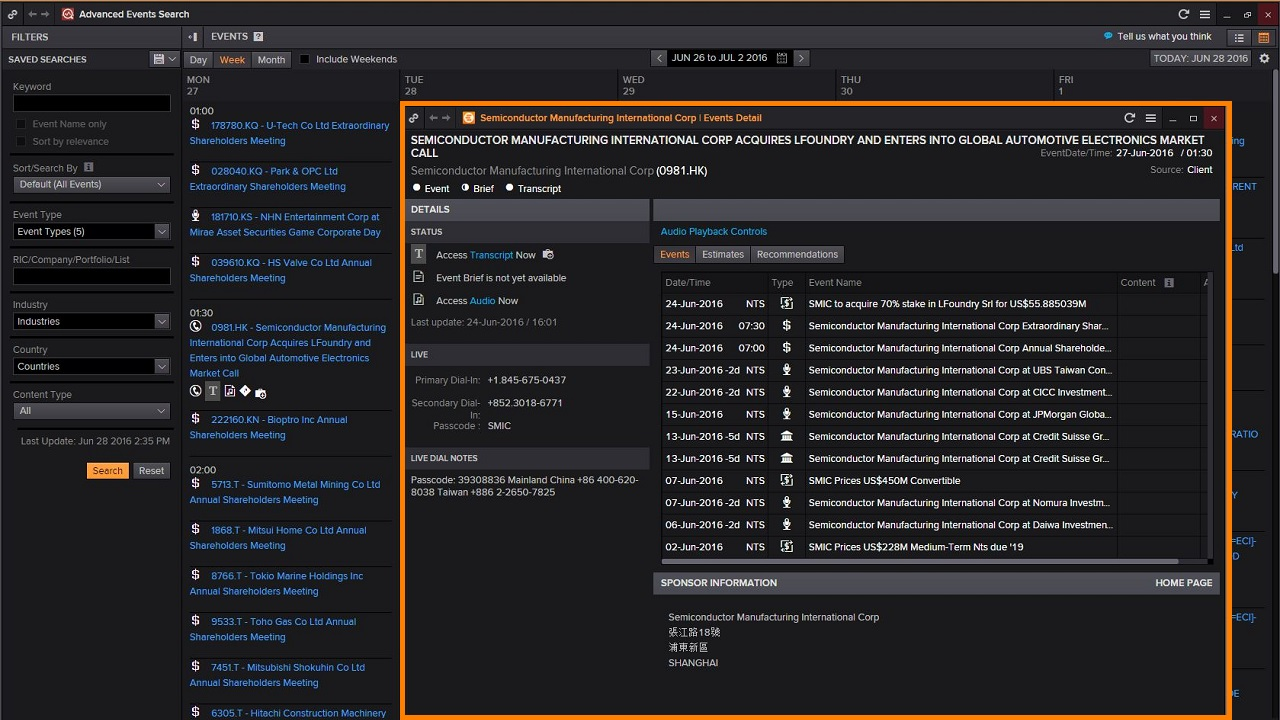
\includegraphics[width=\textwidth]{images/company-events-coverage-eikon.jpg} 
    \caption{Conference call event information in Eikon.}
    \label{fig:eikon}
  \end{center}
\end{figure}

The dataset which is used for the experiments consist of 24,793 conference calls held by 6,131 firms all over the world. All the calls are in English language. Approximately 80\% of the firms are from English-speaking countries. Earnings calls pertaining to fiscal year 2017 contribute to 68\% of the dataset, 22\% are from 2016 and 5\% each is from 2015 and 2018. 
The conference calls are one-hour long conversations with the initial part of the call consists of a presentation about the firm's financials in the previous period and the rest of the call is a question and answer session with journalists and other analysts. Hence, the dataset has different types of speech, prepared one-sided speech is in the first half of the audio and the rest are more conversational in nature. The speech is mostly in the sphere of finance and business and consists of a lot of jargon from this domain. The dataset has different speech from different English accents. An analysis of the companies' metadata show that the dataset consists of conference calls of companies from 76 countries. Out of the 24793 events, 4822 (around 20\%) are from non-native English-speaking countries. Even among the native English-speaking countries, there is a wide distribution of events between the USA, UK, Australia, New Zealand, etc.

Since there are no publicly available results on this dataset for the task of automatic speech recognition, a portion of it was processed using popular cloud speech to text services to analyse the complexity of the dataset. Azure's\footnote{Speech to Text, Audio to Text Translation, Microsoft Azure \href{https://azure.microsoft.com/en-us/services/cognitive-services/speech-to-text/}{https://azure.microsoft .com/en-us/services/cognitive-services/speech-to-text/}} speech to text service and Google's\footnote{Speech-to-Text: Automatic Speech Recognition, Google Cloud \href{https://cloud.google.com/speech-to-text/}{https://cloud.google. com/speech-to-text/}} speech to text services analysed around 2000 randomly sampled utterances from the BizSpeech dataset. The word error rates (WER) on the two services were 19.74\% and 21.9\% on Azure and Google, respectively. Furthermore, on analysing the word error rates based on the nationality of the companies, from Figure \ref{fig:wer_cloud} we can observe that on Google, there is a drop of 32.7\% in WER and in Azure, the drop is 36.5\% from native to non-native utterances which shows that even the most generalized models can suffer with different speaking conditions. 

\begin{figure}[ht]
  \begin{center}
    % below the size of the figure has been reduced for example
    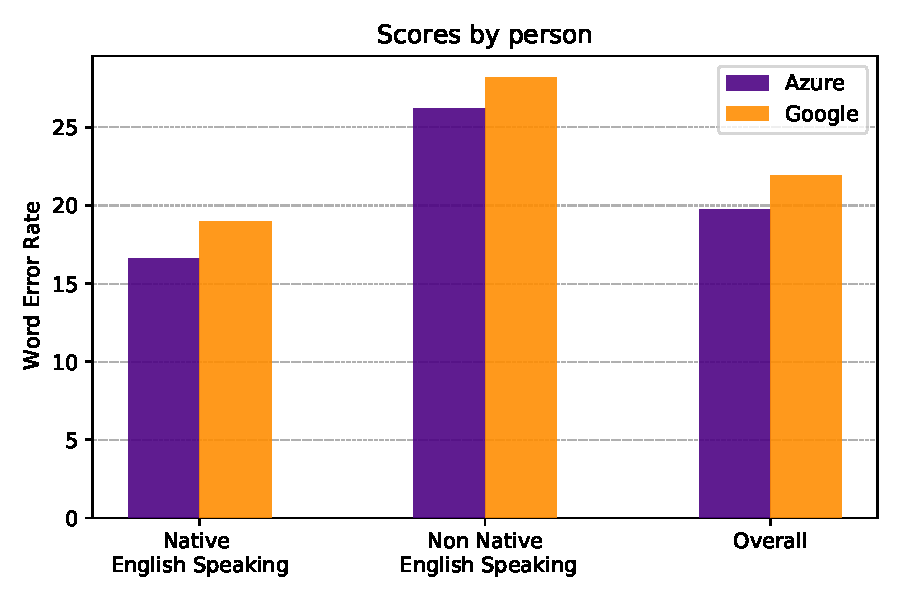
\includegraphics[width=0.8\textwidth]{images/wer_cloud.pdf} 
    \caption{Word Error Rate on Google's and Azure's cloud services.}
    \label{fig:wer_cloud}
  \end{center}
\end{figure}


The main advantage of this dataset is that it is quite a large dataset and includes various speech styles and accents. The drawback of the dataset is that the speech is from a single domain and from a specific field, which might mean that the models trained on this dataset might not be useful for general speech recognition tasks.

The transcript in the dataset consists of text with punctuations and with standard capitalization applied. The dataset consists of non-standard text, like abbreviations, random characters to represent word fillers (like ah, eh, oh.) and many abbreviations and named entities. The phrase "operator instructions" is used in the transcript very frequently to denote that the conference operator is giving out instructions pertaining to the call, and the actual phrase is not present in the audio at all. These inconsistencies (examples shown in Table \ref{table:examples}) make the dataset harder to train and since the size of the dataset is large, it is hard to know where and what other inconsistencies are present in the dataset. 

\begin{table}[ht]
\begin{tabular}{ l p{9.6cm} c c }

 \hline
 \multicolumn{2}{c}{\textbf{Punctuation}} \\
 \hline
 \textbf{Transcript:} & \verb|[..] with the short-term dynamics?| \\ 
 \textbf{Verbatim:} & \verb|[..] with the short term dynamics| \\
 \textbf{Model output:} & \verb|[..] with the short-term dynamics?| \\
 \hline\hline

 \multicolumn{2}{c}{\textbf{Capitalization}} \\
 \hline
 \textbf{Transcript:} & \verb|Hi. This is Andy.| \\ 
 \textbf{Verbatim:} & \verb|hi this is andy| \\
 \textbf{Model output:} & \verb|Hi, this is Andy.| \\
 \hline\hline
 
 \multicolumn{2}{c}{\textbf{Abbreviations \& Named Entities}} \\
 \hline
 \textbf{Transcript:} & \verb|[..] a question from Andrew Porteous, HSBC.| \\ 
 \textbf{Verbatim:} & \verb|[..] a question from andrew porteous h s b c| \\
 \textbf{Model output:} & \verb|[..] a question from Andrew Porteous, HSBC.| \\
 \hline\hline
 
 \multicolumn{2}{c}{\textbf{Random characters}} \\
 \hline
 \textbf{Transcript:} & \verb|[..] things are -- [theoretically], good| \\ 
 \textbf{Verbatim:} & \verb|[..] things are eh theoretically good| \\
 \textbf{Model output:} & \verb|[..] things -- theoretically, good| \\
 \hline\hline
 
 \multicolumn{2}{c}{\textbf{Transcript inconsistencies}} \\
 \hline
 \textbf{Transcript:} & \verb|Operator Instructions| \\ 
 \textbf{Verbatim:} & \verb|welcome to the petit home q one results call| \\
 \textbf{Model output:} & \verb|Welcome to the Petit Home Q1 Results Call.|\\
 \hline\hline
\end{tabular}
\caption{\label{table:examples}Examples of non-standard text in the dataset. For each example, we show the ground truth transcript, the verbatim transcript, which is exact audible speech from the audio file, and the ASR model output, which is the output of our trained end to end speech to text model.}
\end{table}


\section{Data Preparation}
\label{section:dataprep}
After downloading the dataset, training \acrshort{asr} models still requires a few preprocessing steps. This section explains these preprocessing steps in more detail. 

The audio recordings in the BizSpeech dataset, are a mix of MP3 and WAV files which have varying sampling rates between 8 kHz, 16 kHz and 32 kHz. We convert all the audio to WAV format with 16 kHz sampling rate to maintain uniformity across the whole dataset.

\subsection{Forced Alignment}
Even though they have transcripts for the speech, most of them lack timestamps for the utterances or are inaccurate. The audio files are also around 1 hour long in length, and hence it would be impossible to use the data for training \acrshort{asr} models without finer and accurate timestamps for the sentences. 

\begin{figure}[ht]
  \begin{center}
    % below the size of the figure has been reduced for example
    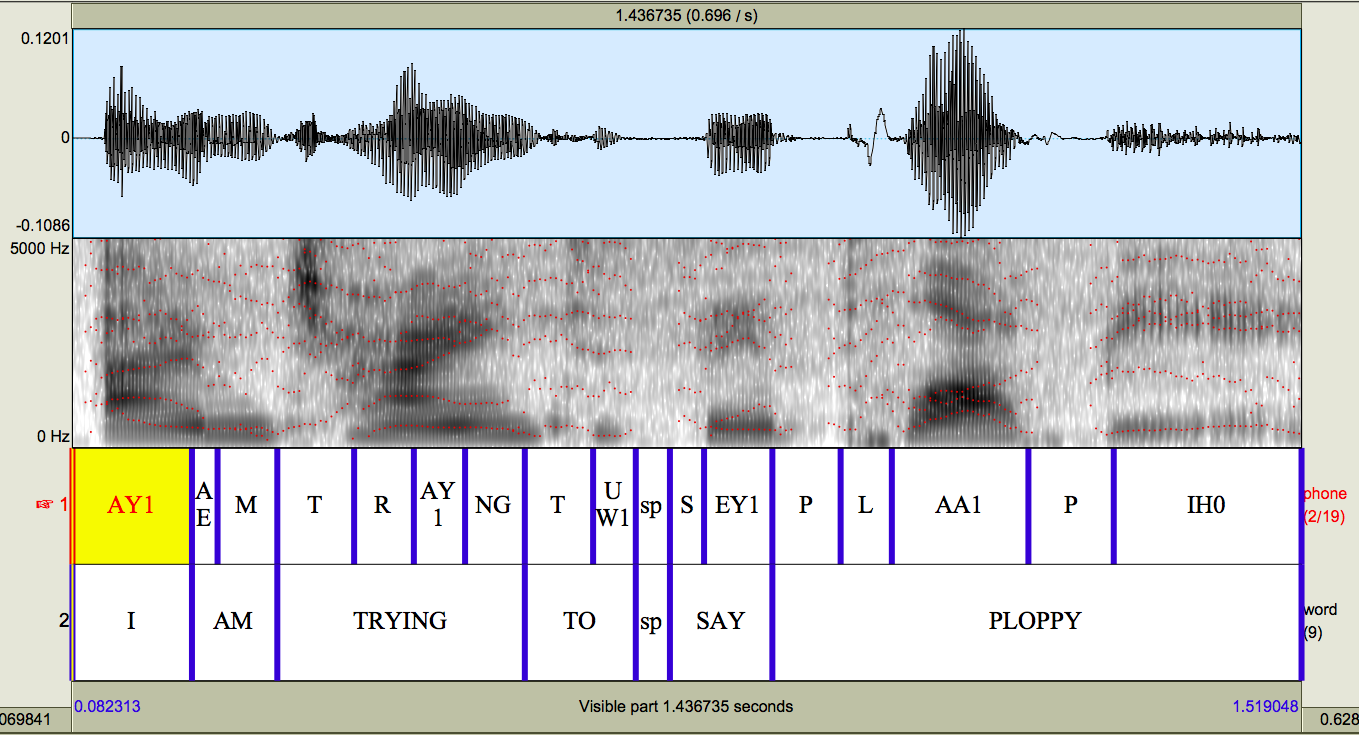
\includegraphics[width=0.8\textwidth]{images/ploppy.png} 
    \caption{Result of forced alignment for an example input. \cite{Yuan2008SPEAKERCORPUS}}
    \label{fig:p2fa}
  \end{center}
\end{figure}

We use forced alignment to generate accurate alignment of speech with the textual data. Forced alignment helps to align linguistic units (e.g., phoneme or words) with the corresponding audio file. It requires an audio file with transcriptions as input, and it outputs the text with word level time-aligned data. We use the P2FA for Python 3\footnote{Penn Phonetics Lab Forced Aligner Toolkit (P2FA) for Python3, \href{https://github.com/jaekookang/p2fa\_py3}{https://github.com/ jaekookang/p2fa\_py3}} tool, which is a \acrshort{hmm} forced aligner based on P2FA \cite{Yuan2008SPEAKERCORPUS} to generate alignments. The aligner works by using a HTK \cite{Young2002TheBook} based acoustic model along with a pronunciation dictionary. The tool generates the transcript's phoneme representation, and then the acoustic model generates accurate time-aligned output. An example of this can be seen in Figure \ref{fig:p2fa}.

As mentioned in their work, the errors for the successful alignments are around 50ms. A risk of using forced aligner is that it always tries to generate some sort of alignment. When any sorts of inconsistencies are present with the text and audio, for example, a missing word in the transcript, they can deceive the tool for the whole file's alignment and the tool fails. It is difficult to automatically detect these cases and a human test is expensive, especially at the scale of the BizSpeech dataset. Due to this issue, \emph{the usable data from the 24,793 audio hours for training \acrshort{asr} model is finally 19973 hours with close to 9 million utterances with a composition of 52,484 speakers.}

\subsection{Data Loading Performance}
Now that accurate time alignments are available for the dataset, we split the large audio files into smaller files such that each audio split has one sentence in it. Each one of these splits is linguistically a sentence, and we label them as an individual utterance and store as a WAV file. We store the text for the utterance in a JSON file along with a few metadata fields, with a unique utterance ID as the filename for both the audio clip and the JSON file. 


Each utterance length ranges from one second up to 60 seconds. Figure \ref{fig:utt_dist} shows the distribution of the utterance length for the whole dataset. We can see that most of the utterances are around the 6-second length. Since, the utterances are small in relative to the overall size of the dataset (close to 20,000 hours) there are about 9 million audio files and 9 million JSON files to be loaded for every training run. This becomes highly inefficient\footnote{Small files, Aalto scientific computing \href{https://scicomp.aalto.fi/triton/usage/smallfiles/}{https://scicomp.aalto.fi/triton/usage/ smallfiles/}} and will lead to problems on opening too many files on the training node. The size of the dataset is also around 5 TB, which makes it hard to store on a single disk storage. Hence, we cannot depend on storing the data on the local SSD drive. All these problems lead to extremely high usage of disk storage, disk I/O usage, network costs (especially for multi node training), and high CPU usage to access and read a high number of files. 


\begin{figure}[ht]
  \begin{center}
    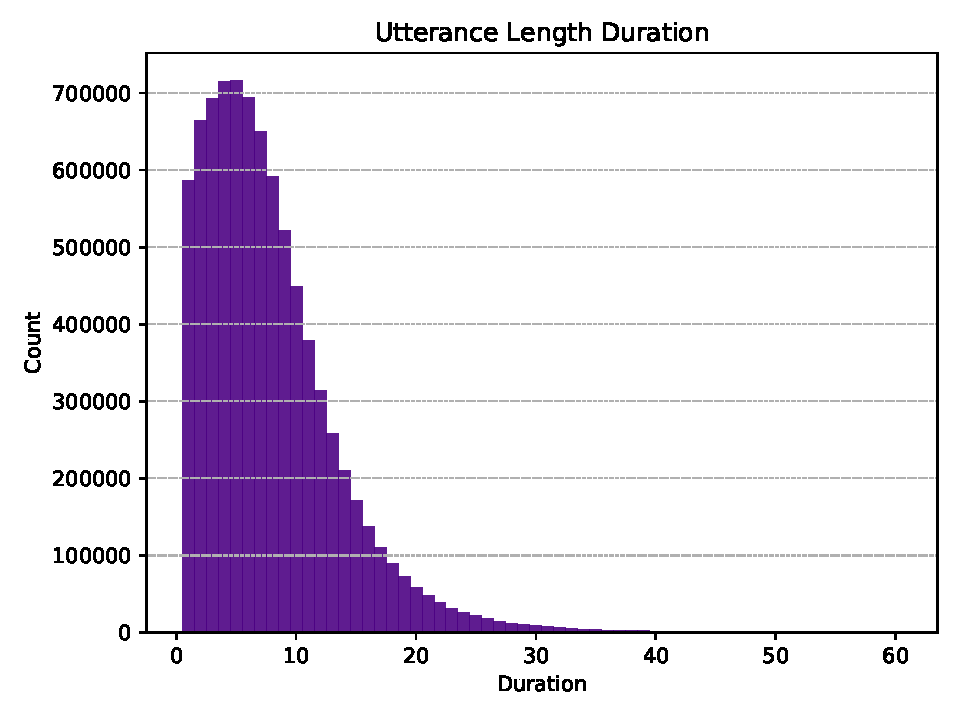
\includegraphics[width=\textwidth]{images/duration_distribution.pdf} 
    \caption{Utterance Duration Distribution for BizSpeech Dataset}
    \label{fig:utt_dist}
  \end{center}
\end{figure}

Hence, we use WebDataset\footnote{webdataset/webdataset: A high-performance Python based I/O system for large (and small) deep learning problems, with strong support for PyTorch. \href{https://github.com/webdataset/webdataset/}{https://github.com/ webdataset/webdataset/}}\cite{Aizman2019HighLearning}, a PyTorch Dataset (\inlinecode{IterableDataset}\footnote{torch.utils.data, PyTorch 1.9.0 documentation \href{https://pytorch.org/docs/stable/data.html}{https://pytorch.org/docs/stable/data .html}}) implementation which provides high efficiency access to data stored in TAR\footnote{GNU tar 1.34: Basic Tar Format \href{https://www.gnu.org/software/tar/manual/html_node/Standard.html}{https://www.gnu.org/software/tar/manual/html\_ node/Standard.html}} archives. This uses only sequential/streaming data access, which brings substantial performance advantage. Figure \ref{fig:seq} shows, on the left side, a file-based access to resources and on the right side, an illustration of sequential based access to resources. We can see from the illustration that sequential data access is much faster and requires much lesser communication. Typically, a ten-fold increase in performance can be seen during I/O operations\cite{Aizman2019HighLearning} for a single node setup with sequential access. This enables large-scale training. Because, it supports basic TAR archives the other advantage is that it becomes easy to create, manage and distribute the data for deep learning training. Since, TAR can be compressed using gzip\footnote{gzip, Wikipedia \href{https://en.wikipedia.org/wiki/Gzip}{https://en.wikipedia.org/wiki/Gzip}} and this is supported directly by webdataset and this helps to save storage space as well. Webdataset can also be set up to use sharding. Sharding helps achieve high throughput using parallel I/O with multiprocess enabled tasks like data loading, preprocessing, etc. This. We specify the shards as a list of files to webdataset, or they can be written using the brace notation. For example, \inlinecode{bizspeech-shard-\{000000..003000\}.tar} means there are 3000 shards. When used with a standard Torch \inlinecode{DataLoader}, this will perform parallel I/O and preprocessing. 


\begin{figure}[ht]
  \begin{center}
    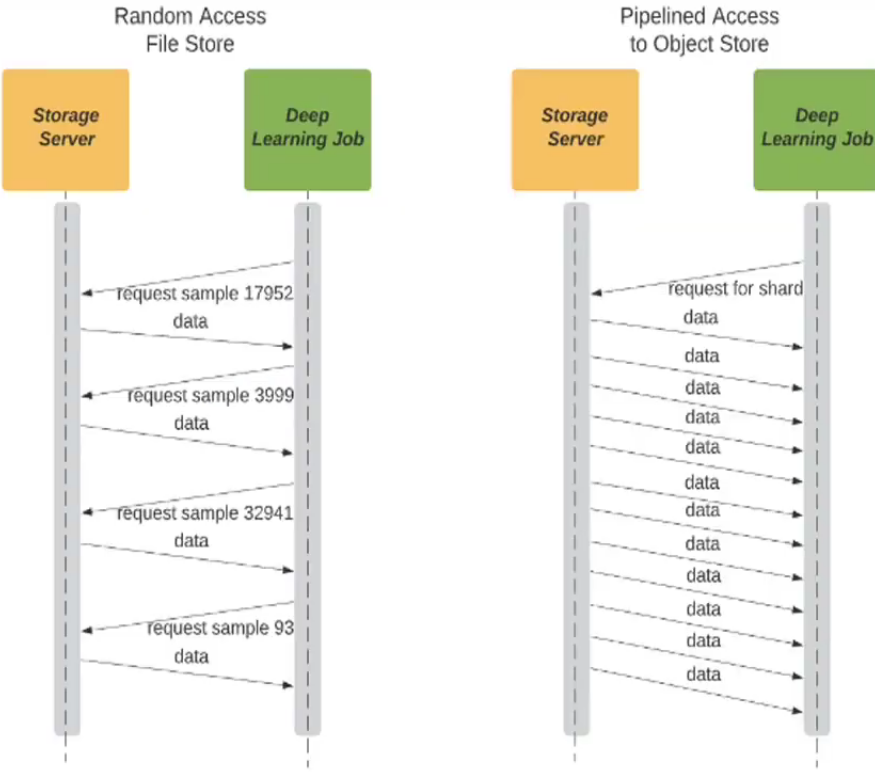
\includegraphics[width=0.7\textwidth]{images/sequential.png} 
    \caption{File-based Access vs Sequential Data Access \cite{Aizman2019HighLearning}}
    \label{fig:seq}
  \end{center}
\end{figure}

\emph{We convert the BizSpeech dataset  to compressed tar to enable usage of webdataset. Split the dataset into 3000 shards, with each shard containing about 700 MB of data after compression, totalling at around 2.1TB storage footprint. This dataset is now ready to be used for training ASR models efficiently. Empirically, speed-up after using webdataset with a single process was around 7-8 fold during training a small subset of 80 hours of the dataset. It becomes very difficult practically to store and test the file-based mechanism to measure the throughput difference for very large-scale experiments. For all the large-scale experiments of order more than 200 hours, we use a configuration of 2-4 worker processes per GPU with sharding and randomization enabled.}

\section{Training Attention based Encoder-Decoder model}
\label{section:attention_train}
For training a speech to text model on BizSpeech dataset, we use SpeechBrain (introduced in Section \ref{section:sb}). SpeechBrain provides recipes which are designed and further optimized for particular datasets. Considering the scale of experiments, we use the LibriSpeech recipe\footnote{speechbrain/recipes/LibriSpeech/ASR/seq2seq \href{https://github.com/speechbrain/speechbrain/tree/develop/recipes/LibriSpeech/ASR/seq2seq}{https://github.com/speechbrain/spee chbrain/tree/develop/recipes/LibriSpeech/ASR/seq2seq}} as a starting point for our experiments. After data loading and preprocessing to parse the audio and transcript text, we generate features from the audio signal. We use logarithmic, mel-based, filter banks 
\cite{Vetterli1992WaveletsDesign} with  0-8000 Hz frequency and the processing happens on-the-fly with data loading. These steps can be parallelized easily by enabling multiprocessing to increase the number of available workers loading the data. From the recipe, we disable the Language Model for our experiments because the focus is on scaling up the training of speech to text and not necessarily to make the model the most accurate one. The final model and configuration used is given in the Appendix \ref{chapter:model-architecture}. We use the negative log likelihood loss function along with the CTC loss (described in Section \ref{section:ctc}) for the initial 15 epochs. 

\subsection{Dynamic Batching}
\label{section:dynbatch}
A problem in automatic speech recognition is when batching up the utterances for training, the varying lengths of utterances means that the shorter utterances have to be padded up to the length of the longest utterance in the batch. Depending on the ordering of the utterances, the batches of data used for training could be high in sparsity due to padding. Because the ordering of training data is usually random, a fixed batch size can be inefficient when the utterances are short. To counter this, we sort the speech data in length to make the \acrshort{gpu} usage more efficient. However, this may affect the model convergence based on the type of ordering used. To solve these problems, SpeechBrain uses dynamic batch data loader where it reads the audio samples to the memory buffer. It then clusters the audio samples based on length and then generates batches of audio samples from similar length utterances, hence avoiding the inefficiencies in data loading due to padding issues. 

\subsection{\emph{Epoch} with dynamic batching}
The data is in random order, and since the data loading workers access the shards asynchronously, it is difficult to keep track of exact epochs (exact epoch here refers to each data sample used exactly once per epoch). Hence, we drop the "one sample per epoch" standard, and instead use sampling with replacement where we draw a sample completely randomly. Previous experiments have shown that sampling by replacement is as good as or in some cases better than one sample per epoch strategy \cite{Recht2012BeneathConsequences, Nielsen2015NeuralLearning}. Tracking the training progress generally involves observing the loss values and accuracy metrics of a validation step after every epoch of training, and since with the newer approach, traditional "epochs" are inconsequential, we track the number of updates to the model. We run the validation step after every 5000 updates to the model. Henceforth, \emph{epoch} refers to 5000 updates to the model and this is used to track training progress using validation loss and validation \acrshort{wer}.

\section{Distributed training}
\label{section:di}
We use two different methods of Multi-GPU training, \acrfull{ddp} is a synchronous, decentralized and as the name suggests, a data-parallel method. Hogwild is an asynchronous, data parallel method. 

\subsection{Synchronous Training}
We use PyTorch's distributed data parallel method to train our model \cite{Li2020PyTorchTraining}. This method enables training in distributed systems by passing gradients before the optimizer step is invoked. This ensures that all model replica parameters are updated using the same gradients, and thus the replicas stay synchronized across all the iterations. Hence, this can be equated to accumulating gradient across multiple batches of data on a single GPU. PyTorch uses \inlinecode{AllReduce} operation which is supported by primitive inter process communication libraries like NCCL\footnote{NVIDIA Collective Communications Library (NCCL), NVIDIA Developer \href{https://developer.nvidia.com/nccl}{https:// developer.nvidia.com/nccl}}, MPI\footnote{Open MPI: Open-Source High-Performance Computing \href{https://www.open-mpi.org/}{https://www.open-mpi.org/}}, etc. The \inlinecode{AllReduce} operation expects a tensor of the same size from all of its participant process and applies a given arithmetic operation, and sends back the output tensor to all the processes involved. It is through this operation that DDP becomes a synchronous method because \inlinecode{AllReduce}  waits until all processes join for a particular iteration, and each individual process waits for the output from \inlinecode{AllReduce} before it moves to the next iteration. More specifically, for implementing DDP for our models, SpeechBrain wraps the models with a \inlinecode{DistributedDataParallel} module from PyTorch. The data loader explained in Section \ref{section:dataprep} scales without any modifications required for a distributed training use-case. We use different processes (can be $>1$ process per replica as well) to load data for the different model replicas.

\subsection{Asynchronous Training}
We implement Hogwild \cite{Niu2011HOGWILD:Descent}, discussed in Section \ref{section:hogwild}. We discuss the parallel processing steps in more details here. We assume a shared parameter model across $p$ processors. The parameters are denoted by $x$ and each process accesses $x$ and can update $x$ because $x$ is stored in shared memory. To update the weights with an update $a$, there is no locking system enforced, so any process can perform the following operation on the shared memory.

$$
x_{v} \leftarrow x_{v}+a
$$

Once the training starts, each processor follows the pseudocode provided in Algorithm \ref{alg:hogwild}. It loads the current state of the model, $x_e$. Let $G_{e}(x)$ denote a gradient of the function $f_{e}$, as in standard \acrshort{sgd}, for a data point $e$ sampled randomly from the dataset, $E$. $\gamma$ is the step size and controls the magnitude of the gradient update. The gradients are updated directly without blocking the other processes.

\RestyleAlgo{ruled}

\begin{algorithm}
\caption{Hogwild algorithm for each process.}\label{alg:hogwild}
\While{}{
    Sample $e$ uniformly at random from $E$
    
    Read current state $x_e$ and evaluate $G_e(x)$
    
    $x_{v} \leftarrow x_{e}-\gamma G_{e}(x)$
}
\end{algorithm}

Once updated, the loop continues with its next iteration by loading new data and loading newer parameters from the shared memory. Since there is no blocking of the model parameters, sometimes  it could so happen that an update of the parameters is overwritten without being used by any processors at all. Results from \cite{Niu2011HOGWILD:Descent} however show that the training can benefit from the non-blocking nature of the training procedure. This is mainly because of the robustness of \acrshort{sgd} to the random ordering of updates to the parameters. \acrshort{sgd} is invariant to the data order and hence to the order in which the updates to the model are received.

